\documentclass[a4paper,twoside,article,danish,table]{memoir}
\semiisopage \checkandfixthelayout
\XeTeXtracingfonts= 1
\usepackage{babel,microtype,verbatim,threeparttable,amsmath,amssymb,unicode-math,ulem,hyperref,siunitx,mhchem,tikz,pgfplots}
\sisetup{per-mode=symbol}
\microtypesetup{final,verbose=silent}
\usetikzlibrary{mindmap,arrows,positioning,shapes}
\setmainfont[Ligatures={TeX}]{Arno Pro}
\setmathfont{Arno Pro}
\setmathfont{[Asana-Math]}
%\hfuzz=1pt
\usepackage[margin,draft]{fixme}
\fxusetheme{color}

\newcommand{\authorvar}{Carl~Emil~Grøn~Christensen and Mathias~Dannesbo}
\newcommand{\pretitlevar}{0}
\newcommand{\titlevar}{Swagway} 
\newcommand{\subtitlevar}{0} 
\newcommand{\datevar}{\today} 
\newcommand{\subjectvar}{Teknikfag~A:~El}
\newcommand{\classvar}{}  
\newcommand{\teachervar}{}

\makepagestyle{articlehead}
\makeevenhead{articlehead}{}{\titlevar}{}
\makeevenfoot{articlehead}{}{}{\thepage}
\makeoddhead{articlehead}{}{\titlevar}{}
\makeoddfoot{articlehead}{}{}{\thepage}

\usepackage{listings,textcomp}
\lstset{language=[Visual]C++,
  morekeywords={[2]abs,acos,asin,atan,atan2,ceil,constrain,cos,degrees,exp,floor,log,map,max,min,radians,random,randomSeed,round,sin,sq,sqrt,tan,bitRead,bitWrite,bitSet,bitClear,bit,highByte,lowByte,analogReference,analogRead,analogWrite,attachInterrupt,detachInterrupt,delay,delayMicroseconds,digitalWrite,digitalRead,interrupts,millis,micros,noInterrupts,noTone,pinMode,pulseIn,shiftIn,shiftOut,tone,Serial,Serial1,Serial2,Serial3,begin,end,peek,read,print,println,available,flush,setTimeout,find,findUntil,parseInt,parseFloat,readBytes,readBytesUntil},
  keywordstyle={\bfseries\color[rgb]{0,0,1}},
  keywordstyle={[2]\bfseries\color[rgb]{0.8,0.33,0}},
  identifierstyle=\ttfamily,
  commentstyle=\color[rgb]{0.133,0.545,0.133},
  stringstyle=\color[rgb]{0.627,0.126,0.941},
  showstringspaces=false,
  basicstyle=\small\ttfamily,
  numberstyle=\footnotesize,
  numbers=left,
  stepnumber=1,
  numbersep=10pt,
  tabsize=2,
  breaklines=true,
  breakatwhitespace=false,
  upquote=true,
  extendedchars=true,
  literate={æ}{{\ae}}1
    {ø}{{\o}}1
    {å}{{\aa}}1
}

\newcommand{\boarddate}[1]{\textcolor{blue!80!black}{#1}}
\newcommand{\issue}[1]{\textsuperscript{\textcolor{blue!80!black}{\href{https://github.com/neic/Swagway/issues/#1}{\##1}}}}


\begin{document}
% \includepdf{forside.pdf} \clearpage%------------------------ Forside

\begin{center}
  \if\pretitlevar 0
  \else{\Large\pretitlevar\\} \fi
  \textsc{\HUGE\titlevar\\}
  \if\subtitlevar 0
  \else {\Large\subtitlevar\\} \fi
  %\vspace{1em}
  {\LARGE 
  af\\
   \authorvar}\\
 \datevar\\
\end{center}

\vfill
\begin{abstract} %------------------------------ Abstract
  \fxwarning{Skriv resume}
\end{abstract}\vfill
\noindent
\begin{tabular*}{\textwidth}{@{\extracolsep{\fill}} ll}

\end{tabular*}

\thispagestyle{empty}
\clearpage

\chapter*{Forord}\label{chap:for}
Gennem teksten vil der være angivet link til “Issues” på GitHub siden for projektet\footnote{\url{https://github.com/neic/Swagway}}. Disse issues har været brugt som projektstyring samt bugtracker gennem projektforløbet. Links er angivet som i enden af denne sætning\issue{1}. Det er ikke nødvendigt for forståelsen af denne rapport at følge linksne.

\fxwarning{Tak til Steffen LC og Kristian}

\clearpage \setcounter{tocdepth}{1} \tableofcontents \clearpage

\chapter{Indledning}\label{chap:ind}
\section{Problemformulering}

\chapter{Indput}

\section{Sensor}
To sensorere, drift.
\subsection{Sensor hardware}
Pull-up, Bus capasistance, level shifter,
\begin{figure}[htbp]
  \centering
  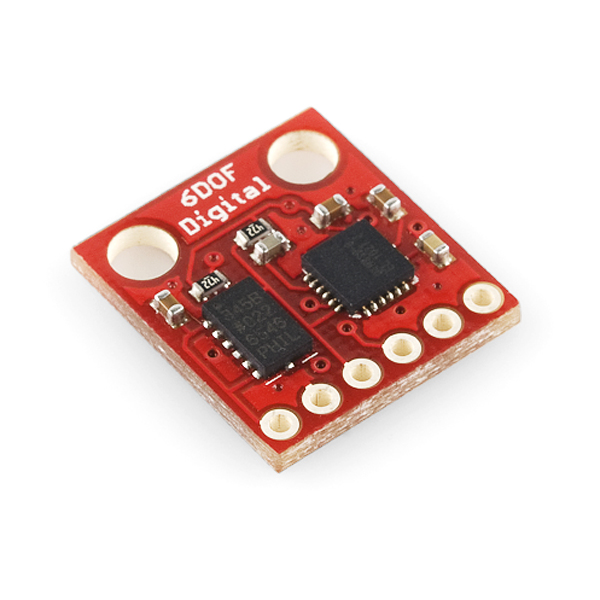
\includegraphics[width=0.3\textwidth]{pictures/imu.jpg}
  \caption[IMU breakoutboard fra Sparkfun]{IMU breakoutboard fra Sparkfun. (CC BY-NC-SA 3.0, Sparkfun)}
  \label{fig:imu}
\end{figure}
\subsection{Sensor software}
I²C, wire.h, libraries

\section{Styring}
Potentiometer, gaffelsensor, strain-gate

\chapter{Control}
\section{Filter}
Mål: samle data fra gyro og acc og regne en vinkel ud
\subsection{Komplimentær filter}
\subsection{Kalman filter}
\subsection{Modificeret kalman filter}

\section{Regulering}
Mål: omsætte en vinkel til en PWM værdi
\subsection{Linær}
\subsection{PID}
\subsection{Eksponential}

\chapter{Output}
Mål: Køre motore i begge retninger med variabel hastighed.
\section{H-broens virkemåde}
H-bro teori
\section{PWM}
PWM teori
\section{Overvejelser}
Vores valg: Dobbelt H-bro med mange chip eller bygge selv. Med eller uden PWM “i bunden”.
\section{Motorcontroller}

\begin{table}[htbp]
  \caption{Motorcontroller sandhedstabel}
  \centering
  % \begin{threeparttable}
  \begin{tabular}{ccc|cccc|ccccl}
    \toprule
    \multicolumn{3}{c}{Arduino pin}&\multicolumn{4}{c}{HEXFET spænding}&\multicolumn{4}{c}{HEXFET on/off}\\
    P7&P6&P5 &Q1&Q2&Q3&Q4 &Q1&Q2&Q3&Q4\\
    P8&P9&P10 &Q5&Q6&Q7&Q8 &Q5&Q6&Q7&Q8\\
    \midrule
    0&0&0 &0&1&0&0 &0&0&0&1 & Off ($\circlearrowright$)\\
    1&0&0 &0&0&0&1 &0&1&0&0 & Off ($\circlearrowleft$)\\
    0&1&0 &1&1&0&0 &1&0&0&1 & $\circlearrowright$\\
    1&1&0 &1&0&0&1 &1&1&0&0 & Short\\
    0&0&1 &0&1&1&0 &0&0&1&1 & Short\\
    1&0&1 &0&0&1&1 &0&1&1&0 & $\circlearrowleft$\\
    0&1&1 &1&1&1&0 &1&0&1&1 & Short\\
    1&1&1 &1&0&1&1 &1&1&1&0 & Short\\
    \bottomrule
  \end{tabular}
  % \begin{tablenotes}
  % \end{tablenotes}
  % \end{threeparttable}
  \legend{Tabellen viser hvordan motorcontrolleren opføre sig hvis den får inputtet angivet under “Arduino Pin”}
  \label{tab:sandhed}
\end{table}

H-bro, PWM, PWM-kondensator, beskyttelses dioder, 4000 serie, optocopler

\subsection{Samlet board}
Det var uparktisk at have alle funktioner på samme board. H-broerne og optocouplerne blev flyttet på sit eget board “Motorcontroller v1.0”.

\subsection{Motorcontroller v1.0}
\boarddate{24. januar 2012}
\fxwarning{Indset diagram over Motorcontroller v1.0}
\fxwarning{Indset figur over Motorcontroller v1.0}
Boardet virkede ikke. Det opførte sig som det var kortsluttet. Det viste sig, efter at boardet var skilt helt af igen, at det plus tegn der skulle vise polariteten var sat ved den forkerte pol. Printet havde taget skade af at blive loddet på flere gange.

Der var desuden nolge ledninger der var for tætsiddene og loddeøerne var lidt underdimmentionerede. Der manglede også en mulighed for at se hvilken vej strømmen løber i H-borerne. Dette blev rettet i v2.0.
\subsection{Motorcontroller v2.0}
\boarddate{8. marts 2012} Dette board blev aldrig lavet færdig; Ledningerne omkring pinheaderen var for tæt efter at loddeøeren blev forstørret. Diagram og figur over printet kan findes i bilag. \fxwarning{ref}

\subsection{Motorcontroller v2.1}
\boarddate{8 marts 2012}

\fxwarning{Indset diagram over Motorcontroller v2.1 (Figur over printet kan findes i bilag)}

Boardet fungerede umiddelbart. Motoren kunne køre i begge retninger og farten kunne styres med PWM. Dog startede motoren på ca. 30\% fart i den ene retning. Ved at måle på PWM signalet fra mainboardet og signalet til motoeren kunne problemet indskrenkes til at være på Motorcontrolleren.

Det viste sig efter meget debugging at spændingen på gaten på P-kanal HEXFETerne (IRF4905) ikke gik high ligeså hurtigt som forventet. Der blev opstillet et forsøg på et breadboard med en P-kanal HEXFET, en optocoupler og en Arduino.

\fxwarning{Indset diagram over forsøg med optocoupler og HEXFET}

Forsøget viste at når optocoupleren sad mellem HEXFETen og Arduinoen var der en kapacitet mellem HEXFETens gate og source. Figur \ref{fig:stigetid} viser nederst PWM signalet fra Arduinoen og øverst signalet på P-kanal HTXFETens gate. Man ser tydeligt at det tager ubelejligt før signalet på gaten stiger.
\begin{figure}[htbp]
  \centering
  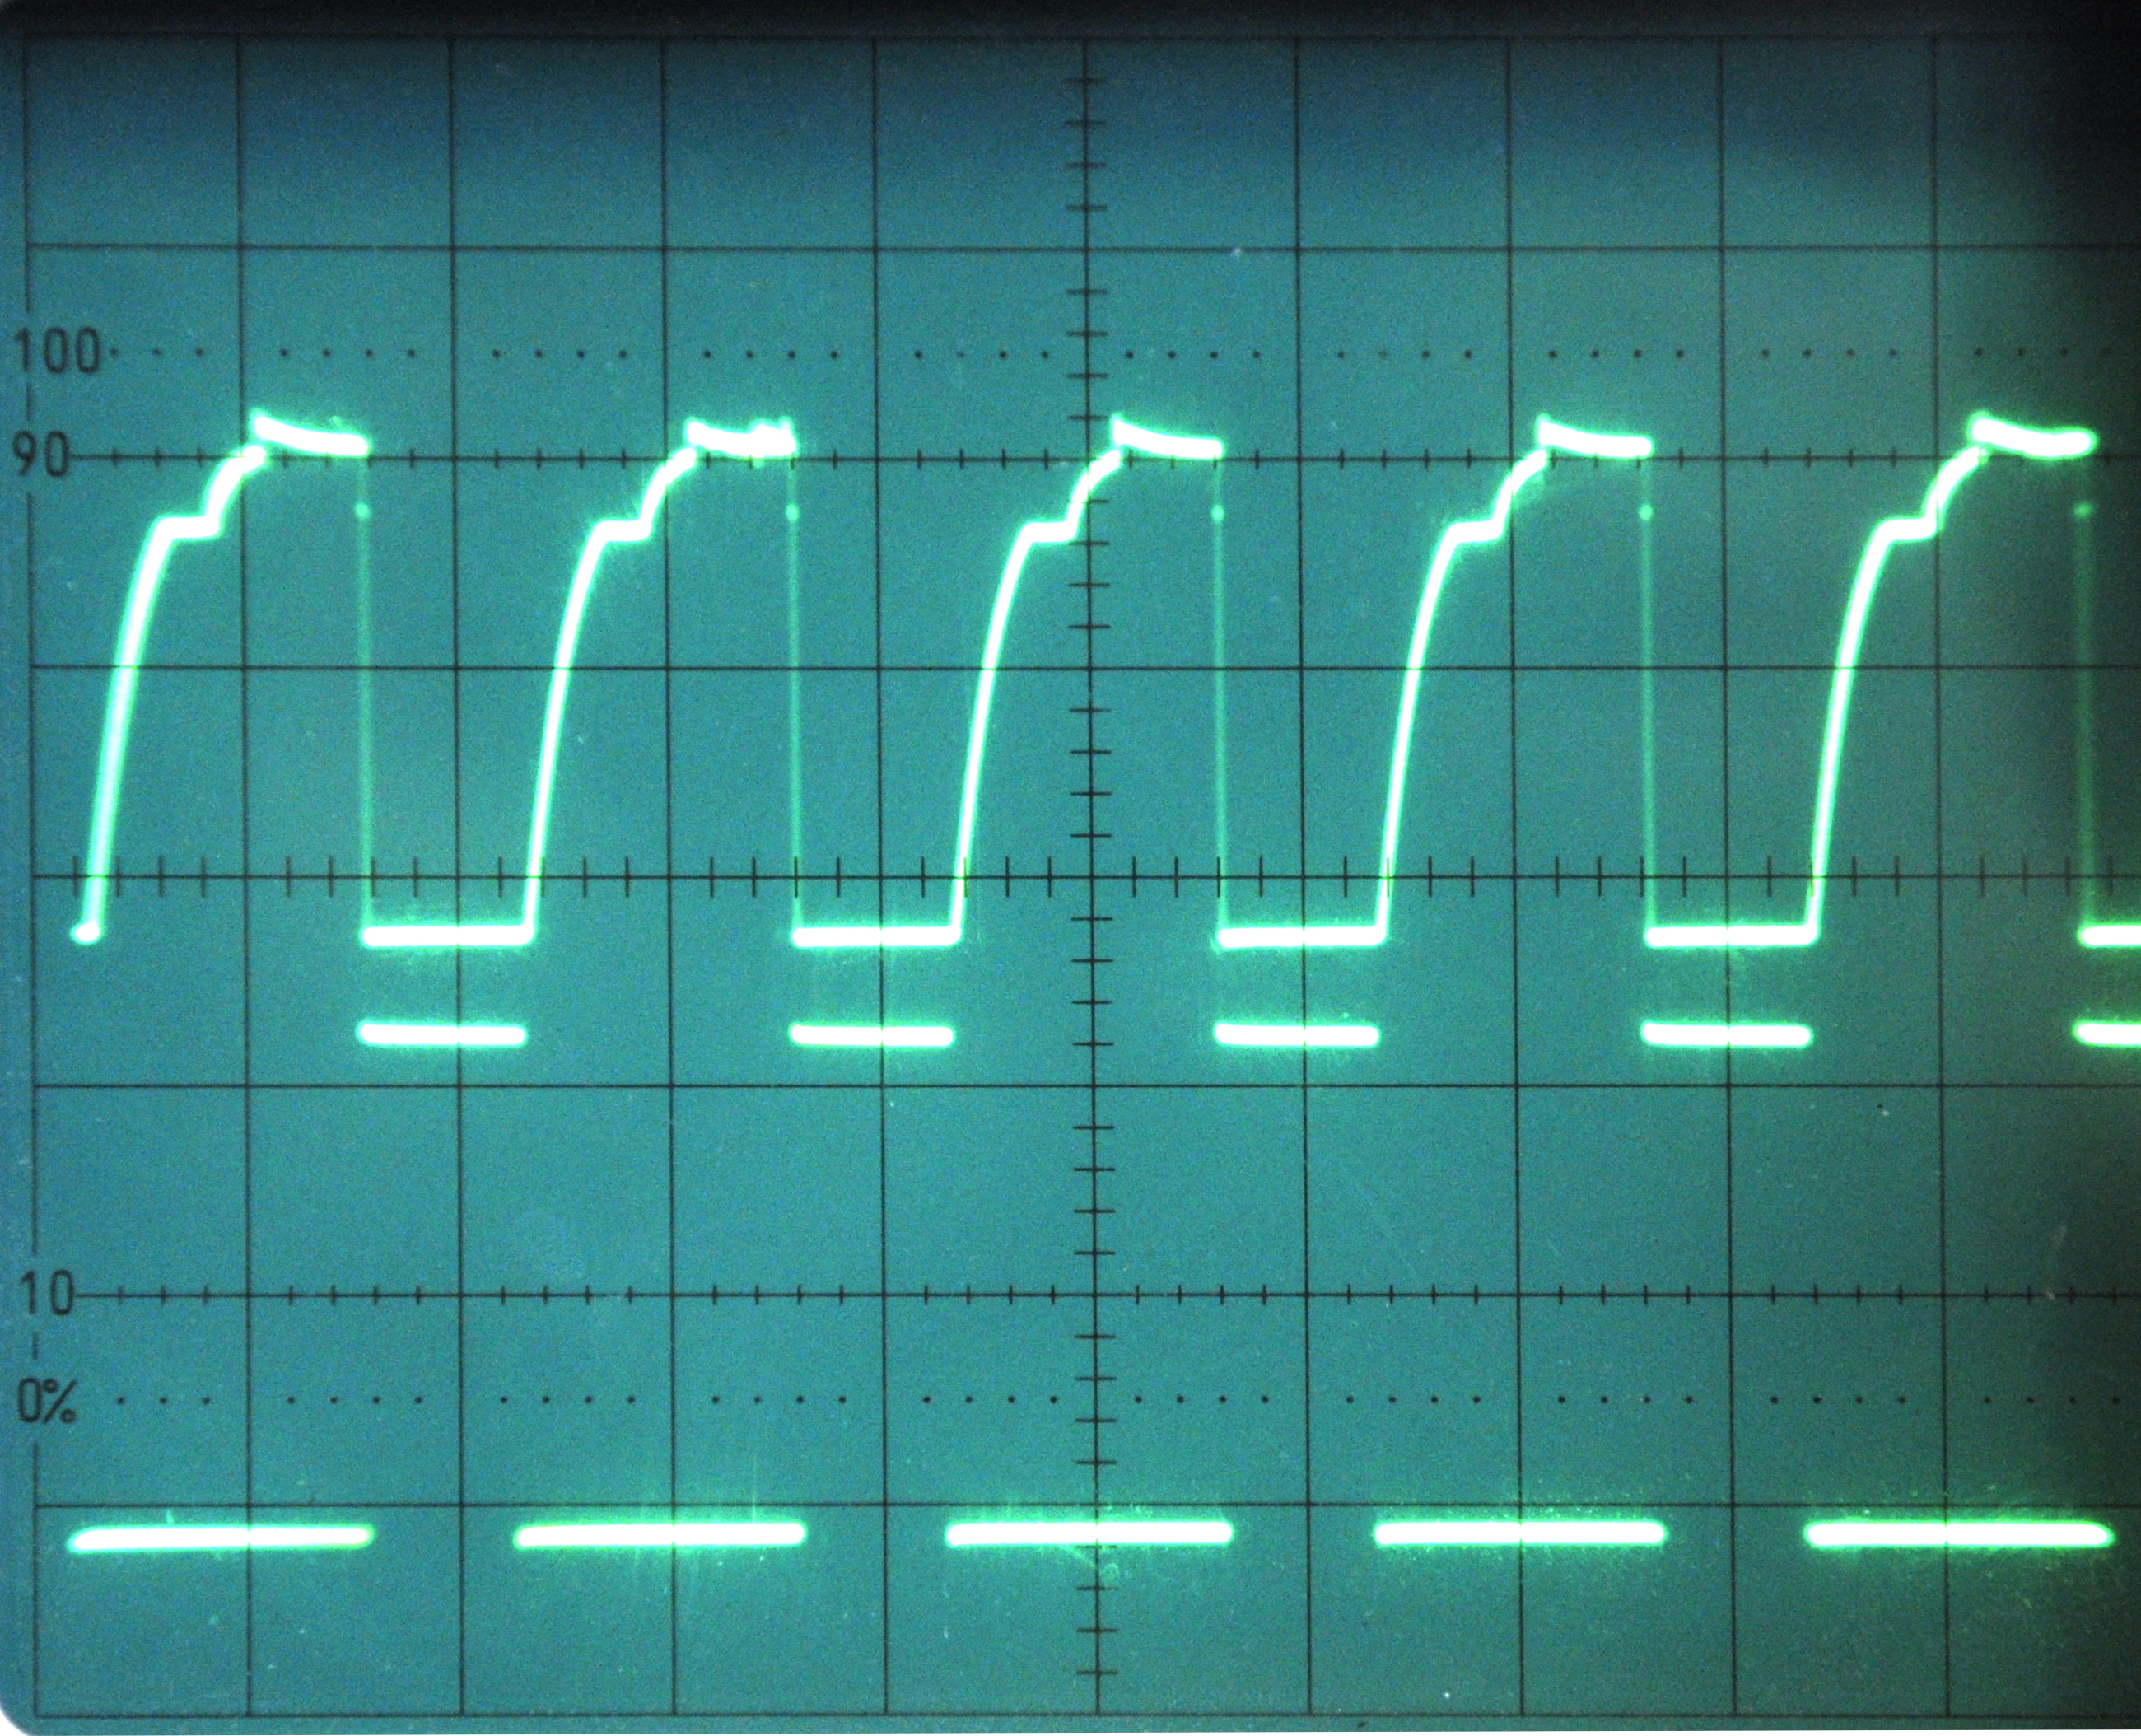
\includegraphics[width=0.8\textwidth]{pictures/stigetid.jpg}
  \caption[Oscilloskop billede af stigetid på en P-kanal HEXFET gate]{Oscilloskop billede af stigetid på en P-kanal HEXFET gate. Nederst ses PWM-signalet fra Arduinoen, øverst ses signalet på gaten.}
  \label{fig:stigetid}
\end{figure}

Ved at sætte en mindre pull-up-modstand på kunne den aflades hurtigere, men det var ikke muligt at få den tilpas langt ned til at kunne styre motoren godt. Ved at fjerne optocoupler og køre HEXFETens gate direkte fra Arduinoen eller ved fjerne HEXFETen og måle direkte på optocoupleren, var stigningstiden $\approx0$. Det var kun i kombination mellem HEXFETen og transistoen i optocoupleren at stigningstiden ikke var $\approx0$.

Der blev forsøgt med en 4N25 optocoupler istedet for 4N35 og en BC547 istedet for optocoupleren; der var samme stigningstid.

Det har ikke været muligt, selv med hjælp fra vejleder, at forklare hvorfor denne kapacitet er der.

Problemet blev ikke løst, det blev bare gjort ubetydeligt: Istedet for at bruge en N- og en P-kanal HEXFET til at bestemme retning og køre PWM på de andre to N- og P-kanal HEXFETer, blev det lavet om til at begge P-kanal HEXFETer blev brugt til at bestemme retning og at N-kanal HEXFETerne bliver brugt at køre PWM. Det er ikke et problem at stigetiden på P-kanal HEXFETerne er langsom da de kun ændre sig når der skiftes retning og ikke med høj frekvens som ved PWM.

For ikke at tilføje flere optocouplere og bruge flere pins på arduinoen blev der, på Motorcontrolleren tilføjet to invertere. Se figur \fxwarning{ref: dia:v3.0}
\subsection{Motorcontroller v3.0}
\boarddate{27. marts 2012}
\fxwarning{Indset diagram over Motorcontroller v3.0 (Figur over printet kan findes i bilag)}
Efter at der blev tilføjet en inventere på to af gatesne til P-kanal HEXFETerne er denne low når der ikke er spænding på optocouplerne (fx når den ikke er koblet til Mainboardet). Det tænder HEXFETen, det, sammen med N-kanal HEXFETerne som også er tændt uden spænding på optocouplerne, kortslutter H-broen. Motorcontroller v3.0 var fungerede, men det var upraktisk at den var kortsluttet unden at være koblet sammen med Mainboardet.

Pull-up modstandende blev erstattet af pull-down.
\subsection{Motorcontroller v4.0}
\boarddate{12. april 2012} Dette board blev aldrig lavet færdig. En stor del af boardet blev re-routed da der var blevet rodet efter mange versioner. Diagram og Figur over printet kan findes i bilag. \fxwarning{ref}

\subsection{Motorcontroller v4.1}
\boarddate{13. april 2012}
Der var en ledning der ikke var routed og der var nogle mindre re-routing.

\subsection{Motorcontroller v4.2}
\boarddate{17. april 2012} Dette board blev aldrig lavet færdig.
Formodstandene til optocouplerne blev flyttet fra mainboardet til Motorcontrolleren.

\subsection{Motorcontroller v5.0}
\boarddate{24. april 2012} Dette board blev aldrig lavet færdig.
Der blev tilføjet LEDer til optocouplerne så man kan se hvornår de er tændt.  

\subsection{Motorcontroller v5.1}
\boarddate{24. april 2012} Dette board blev aldrig lavet færdig.
Nogle pins blev flyttet i fladkablet. 

\subsection{Motorcontroller v5.2}
\boarddate{24. april 2012}
\fxwarning{Board brænder af}
\begin{figure}[htbp]
  \centering
  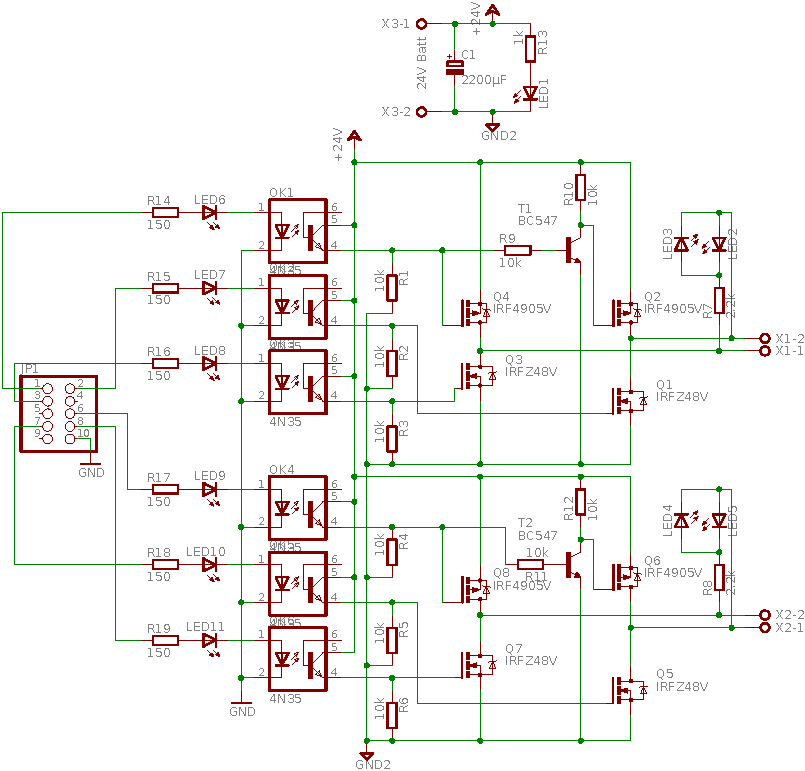
\includegraphics[width=\textwidth]{pictures/MotorcontrollerSch5-2.pdf}
  \caption{Diagram over Motorcontroller v5.2}
  \label{fig:sch5.2}
\end{figure}

Dette board fungere og sidder i Swagwayen.

\subsection{Motorcontroller v6.0}
\boarddate{24. april 2012}

\chapter{Auxiliary}
\begin{table}[htbp]
  \caption{Pin forbindelser på Arduino}
  \centering
  \begin{threeparttable}
    \begin{tabular}{rll}
      \toprule
      Pin & Forbindelse & Egenskaber\\
      \midrule
      0 & USB Rx & \\
      1 & USB Tx & \\
      2 & Radio Rx & Interrupt\\
      3 & & Interrupt, PWM\\
      4 & Radio Tx & \\
      5 & Motorcontroller R2 & PWM\tnote{a}\\
      6 & Motorcontroller L2 & PWM\tnote{a}\\
      7 & Motorcontroller L1 & \\
      8 & Motorcontroller R1 & \\
      9 & Motorcontroller L3 & PWM\\
      10 & Motorcontroller R3 & PWM\\
      11 & & PWM\\
      12 & & \\
      13 & & LED\\
      A0 & & \\
      A1 & & \\
      A2 & Steering & \\
      A3 & Steering & \\
      A4 & IMU I²C SDA & SDA\\
      A5 & IMU I²C SCL & SCL
    \end{tabular}
    \begin{tablenotes}
      \item[a]{PWM outputtet fra disse er lidt højere end forventet. De drives af en anden timer\issue{42}. Se under Mainboard 4.0 i sektion.\ref{sec:main40}}
    \end{tablenotes}
  \end{threeparttable}
  % \label{tab:}
\end{table}

\section{Mainboard}

\subsection{Mainboard v1.0}
\boarddate{24 jan 2012}
Loddeøerne var underdimmentioneret\issue{1} og det var ikke til at komme til at trykke på resetknappen på Arduinoen da bordet dækkede overdet\issue{2}. Der blev tilføjet en resetknap på mainboardet samt et stik til at læse data fra styret\issue{12}.

\subsection{Mainboard v2.0}
\boarddate{1 marts 2012}
Logik kredsløbet blev opgivet og efterfølgende blev der brugt tre Arduino pins per motor\issue{21}. Displayboardet blev ligeledes opgivet\issue{9}. Pinheaderne til 9V og IMUen var desuden for tæt sammen\issue{13}.

\subsection{Mainboard v3.0}
\boarddate{26 marts 2012} Dette board blev aldrig lavet færdig.
Tilføjet pins til radio\issue{29}.

\subsection{Mainboard v3.1}
\boarddate{29 marts 2012}
Formodstandene til optocouplerne på motorboardet blev flyttet til motorboardet\issue{37}.
Pinheaderen til IMUen blev lavet om fra 2×7 til 2×5

\subsection{Mainboard v4.0}\label{sec:main40}
\boarddate{24 april 2012}
Swagwayen kører med dette board, men den ene motor kørte hurtigere end den anden\issue{42}. Det lignede umiddelbart en mekanisk fejl, men ved at bytte om på ledningerne til motorene viste det sig at den ene kanal på kotorcontrolleren kørte langsommere end den anden. Problement blev isoleret til at Arduinoen ikke sendte PWM med samme frekvens til begge kanaler. I Arduino referencen for \texttt{AnalogWrite()} ser man også at pin 5 og 6 PWM kører fra en anden timer end de andre PWM pins. Tilfældigvis kørte den ene motor på begge af disse pins. Pin 5 og 9 blev byttet så Swagwayen kører lidt hurtigere forlens end baglens, men med samme forskel på begge hjul.

Opbytningen af de to pins blev gjort ved at bryde kobberbanerne på printet og lodde to ledninger på, der blev ikke lavet et nyt board.

\chapter{Mekanik}
Motorer, batterier, 
\chapter{Konklusion} \label{chap:kon}
Vi satte os de og de mål, vi nåede de og de mål.

\chapter{Perspektivering} \label{chap:per}
Styring
Kraftigere motorer med mindre gearkasser.
Encodere


\clearpage
\listoftables
\listoffigures
% \nocite{*}
\bibliographystyle{dk-apali} \bibliography{bib}
\clearpage \appendix

\chapter{Kildekode}

\section{\texttt{swagway.ino}}
\lstinputlisting{../Software/swagway/swagway.ino}
\section{\texttt{ADXL345.h}}
\lstinputlisting{../Software/swagway/ADXL345.h}
\section{\texttt{ADXL345.cpp}}
\lstinputlisting{../Software/swagway/ADXL345.cpp}

\chapter{Status log}

\section{13. marts}
Mainbord er fungerende. v2.0 af motorboardet er næsten færdig.

Kredsløbet uden om printne er næsten færdig.

Vi kan læse data fra IMUen og vi har et halvt implementert kalman-filter.

Efter kalmanfilteret fungere skal der implementeres PID med wrapper kode.

\end{document} 